\section{Results}
\subsection{Calibration}

Due to small defects in the construction of the telescope and limitations of the motors of the dish and the antenna, the pointing of the antenna doesn't always line up with the target. It is therefore necessary to calibrate it before pointing at distant objects. The Sun is the strongest discrete radio source in the sky \cite{burke_introduction_2013}, mostly due to black body radiation, and is therefore an ideal target for the calibration.
By configuring the antenna to point towards Sun, using its actual coordinates, and scanning the surrounding area in Az/Alt coordinates, the maximum average measured power gives the real position of the Sun in the specific antenna coordinates. The measured power and a linear interpolation of those values shown in \autoref{fig:calibration_contour} gives a correction to the pointing of
\begin{equation}
    \Delta a = -(5.25 \pm 0.50)^\circ \quad \textrm{and} \quad \Delta h = -(2.70 \pm 0.10)^\circ
\end{equation}
\begin{figure}[htbp]
    \centering
    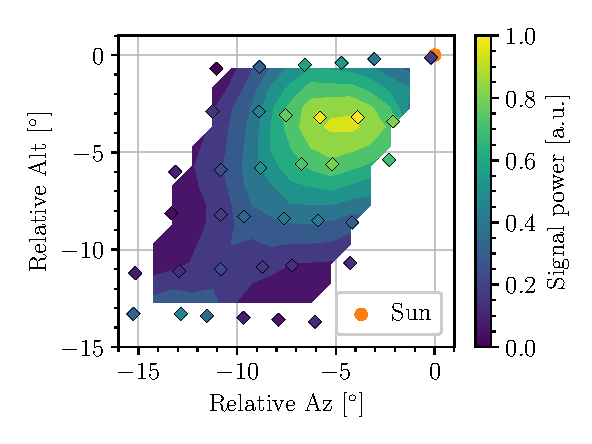
\includegraphics[scale=1]{figures/calibration_contour.pdf}
    \caption{Interpolation of signal power measured in the proximity of the Sun.}
    \label{fig:calibration_contour}
\end{figure}

\subsection{Distinguishing signal and noise}
The signal received by the antenna inherently contains noise which must be removed for the data to be properly analysed.
To this end, a [measure was taken] with the telescope pointed towards a nearby building, so that the registered spectrum  contained only the noise [proper to] the telescope location, which is expected to be found in all the signals received by the antenna.
The spectra of all the subsequently acquired signals were then divided by this noise spectrum, obtaining  signal-to-noise ratios which were further cleaned up by applying a moving average filter \hl{or median in some cases?}.
An example of the application of this pipeline is depicted in \autoref{fig:process_example}.
\begin{figure}
    \begin{subfigure}{0.49\textwidth}
        \centering
        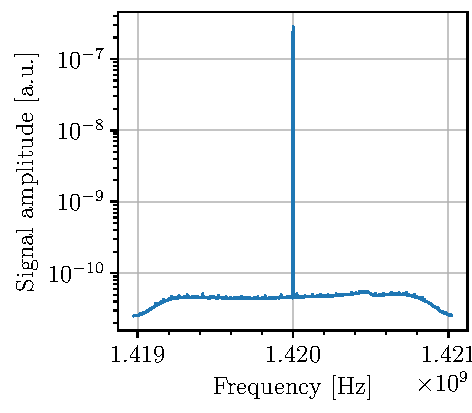
\includegraphics[scale=1]{figures/raw_signal.pdf}
        \caption{}
        \label{fig:raw_signal}
    \end{subfigure}
    \begin{subfigure}{0.49\textwidth}
        \centering
        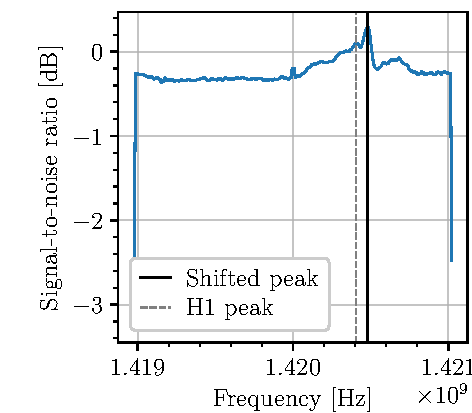
\includegraphics[scale=1]{figures/clean_signal.pdf}
        \caption{}
        \label{fig:clean_signal}
    \end{subfigure}
    \caption{Unprocessed and Processed}
    \label{fig:process_example}
\end{figure}


\subsection{Velocity field of the Milky Way}
Probing arms of milky way

Talk about orientation (i.e. sky visible at measuring time),
We neglect movement of Earth inside solar system.

\begin{figure}[htbp]
    \begin{minipage}[t]{0.5\textwidth}
        \centering
        \captionsetup{width=.9\textwidth}
        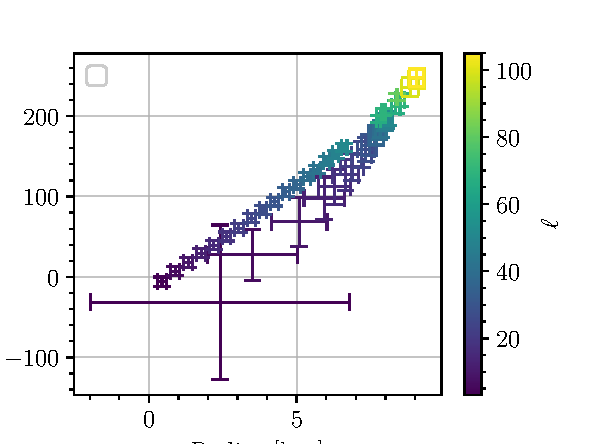
\includegraphics[scale=1]{figures/VEGA_velocity_curve.pdf}
        \caption{Velocity curve VEGA}
        \label{fig:VEGA_velocity_curve}
    \end{minipage}
    \begin{minipage}[t]{0.5\textwidth}
        \centering
        \captionsetup{width=.9\textwidth}
        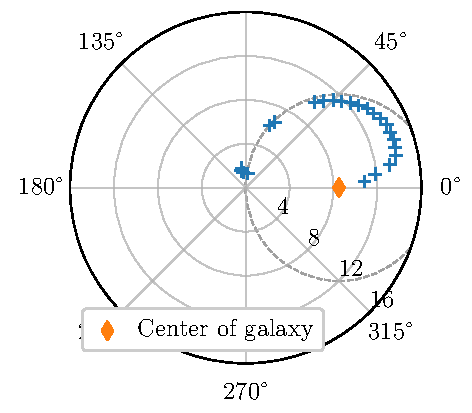
\includegraphics[scale=1]{figures/VEGA_galaxy_map.pdf}
        \caption{Galaxy map VEGA}
        \label{fig:VEGA_galaxy_map}
    \end{minipage}
\end{figure}

\subsection{Comparison with SALSA}
Since VEGA is very young, we compared with a more mature telescope: SALSA, the Torre SRT in Onsala Observatory, Sweden.

Built-in correction for movement of Earth in solar system
\begin{figure}[htbp]
    \begin{minipage}[t]{0.5\textwidth}
        \centering
        \captionsetup{width=.9\textwidth}
        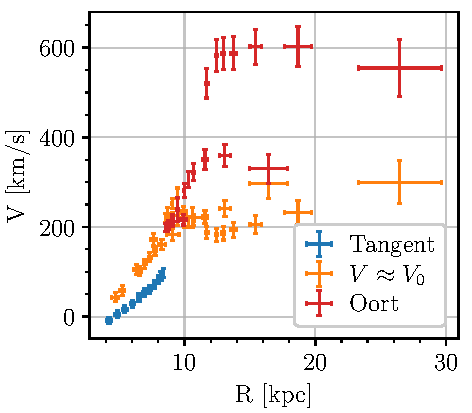
\includegraphics[scale=1]{figures/SALSA_velocity_curve.pdf}
        \caption{Velocity curve SALSA}
        \label{fig:SALSA_velocity_curve}
    \end{minipage}
    \begin{minipage}[t]{0.5\textwidth}
        \centering
        \captionsetup{width=.9\textwidth}
        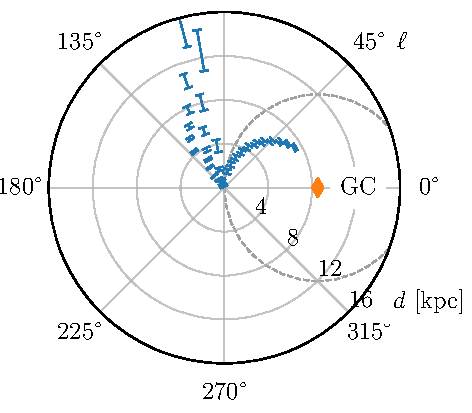
\includegraphics[scale=1]{figures/SALSA_galaxy_map.pdf}
        \caption{Galaxy map SALSA}
        \label{fig:SALSA_galaxy_map}
    \end{minipage}
\end{figure}